% !TEX program = xelatex

%\title{LaTeX Portrait Poster Template}
%%%%%%%%%%%%%%%%%%%%%%%%%%%%%%%%%%%%%%%%%
% a0poster Portrait Poster
% LaTeX Template
% Version 1.0 (22/06/13)
%
% The a0poster class was created by:
% Gerlinde Kettl and Matthias Weiser (tex@kettl.de)
% 
% This template has been downloaded from:
% http://www.LaTeXTemplates.com
%
% License:
% CC BY-NC-SA 3.0 (http://creativecommons.org/licenses/by-nc-sa/3.0/)
%
%%%%%%%%%%%%%%%%%%%%%%%%%%%%%%%%%%%%%%%%%

%----------------------------------------------------------------------------------------
%	PACKAGES AND OTHER DOCUMENT CONFIGURATIONS
%----------------------------------------------------------------------------------------

\documentclass[a0,portrait]{a0poster}

\usepackage{multicol} % This is so we can have multiple columns of text side-by-side
\columnsep=100pt % This is the amount of white space between the columns in the poster
\columnseprule=3pt % This is the thickness of the black line between the columns in the poster

\usepackage[svgnames]{xcolor} % Specify colors by their 'svgnames', for a full list of all colors available see here: http://www.latextemplates.com/svgnames-colors

\usepackage{times} % Use the times font
%\usepackage{palatino} % Uncomment to use the Palatino font

\usepackage{graphicx} % Required for including images
\graphicspath{{pic/}} % Location of the graphics files
\usepackage{booktabs} % Top and bottom rules for table
\usepackage[font=small,labelfont=bf]{caption} % Required for specifying captions to tables and figures
\usepackage{amsfonts, amsmath, amsthm, amssymb} % For math fonts, symbols and environments
\usepackage{wrapfig} % Allows wrapping text around tables and figures

\usepackage{tikz}
\usepackage{rotating}
\usepackage{pgfplots}
\pgfplotsset{compat=newest}
\pgfplotsset{plot coordinates/math parser=false}
\newlength\figureheight
\newlength\figurewidth
\usepackage{tikz}
\usetikzlibrary{decorations.text}

%
%%% \textwidth = 6.5 in
%%% \textheight = 9 in
%%% \oddsidemargin = 0.0 in
%%% \evensidemargin = 0.0 in
%%% \topmargin = 0.0 in
%%% \headheight = 0.0 in
%%% \headsep = 0.0 in
%%% \parskip = 0.2in
%%% \parindent = 0.0in
%
%\newcounter{l2}
%\newcommand{\balphlist}{\begin{list}{(\alph{l2})}{\usecounter{l2}}}
%
%% Theorems
%\newtheorem{theorem}{Theorem}
%\newtheorem{lemma}[theorem]{Lemma}
%\newtheorem{corollary}[theorem]{Corollary}
%\newtheorem{proposition}[theorem]{Proposition}
%\newtheorem{definition}[theorem]{Definition}
%\newtheorem{example}[theorem]{Example}
%\newtheorem{result}{Result}
%\newtheorem{remark}[theorem]{Remark}
%\newtheorem{code}{Code}
%%\newtheorem{algorithm}{Algorithm}
%%\newtheorem{problem}{The Identification Problem}
%\renewcommand{\thm}[1]{\begin{theorem} #1 \end{theorem}}
%\renewcommand{\rem}[1]{\begin{remark} #1 \end{remark}}
%%\newcommand{\lem}[1]{\begin{lemma} #1 \end{lemma}}
%%\newcommand{\cor}[1]{\begin{corollary} #1 \end{corollary}}
%\renewcommand{\prop}[1]{\begin{proposition} #1 \end{proposition}}
%%\newcommand{\defn}[1]{\begin{definition} #1 \end{definition}}
%\newcommand{\ex}[1]{\begin{example}\normalfont #1 \hfill $\Box$ \end{example}}
%%\newcommand{\prf}[1]{\begin{proof}\normalfont #1 \hfill $\blacksquare$ \end{proof}}
%\newcommand{\prf}[1]{{\em Proof:} \, #1 \hfill $\blacksquare$}

%% \newtheorem{proof}% name
%%   {}%      Space above, empty = `usual value'
%%   {}%      Space below
%%   {}% Body font
%%   {\parindent}% Indent amount (empty = no indent, \parindent = para indent)
%% %  {}% Indent amount (empty = no indent, \parindent = para indent)
%%   {\bf}% Thm head font
%%   {:}%        Punctuation after thm head
%%   {}%     Space after thm head: " " = normal interword space;
%%         %       \newline = linebreak
%%   {}% Thm head spec
%% \theoremstyle{proof}




% Numbering
%\numberwithin{theorem}{section}
%\numberwithin{lemma}{section}
%\numberwithin{corollary}{section}
%\numberwithin{proposition}{section}
%\numberwithin{definition}{section}
%\numberwithin{equation}{section}
%\numberwithin{example}{section}
%\numberwithin{code}{section}
%\numberwithin{algorithm}{section}
%\numberwithin{problem}{section}

% Math

\newcommand{\EXP}{\Eset}
\newcommand{\R}{\mathds{R}}
\newcommand{\C}{\mathds{C}}
\newcommand{\F}{\mathds{F}}
\newcommand{\N}{\mathds{N}}
\newcommand{\Q}{\mathds{Q}}
\newcommand{\Z}{\mathds{Z}}

\newcommand{\Aset}{{\mathbb A}}
\newcommand{\Bset}{{\mathbb B}}
\newcommand{\Cset}{{\mathbb C}}
\newcommand{\Dset}{{\mathbb D}}
\newcommand{\Eset}{{\mathbb E}}
\newcommand{\Fset}{{\mathbb F}}
\newcommand{\Gset}{{\mathbb G}}
%\newcommand{\Hset}{{\mathbb H}}
\newcommand{\Iset}{{\mathbb I}}
\newcommand{\Jset}{{\mathbb J}}
\newcommand{\Kset}{{\mathbb K}}
\newcommand{\Lset}{{\mathbb L}}
\newcommand{\Mset}{{\mathbb M}}
\newcommand{\Nset}{{\mathbb N}}
\newcommand{\Oset}{{\mathbb O}}
\newcommand{\Pset}{{\mathbb P}}
%\newcommand{\Qset}{{\mathbb Q}}
%\newcommand{\Rset}{{\mathbb R}}
\newcommand{\Sset}{{\mathbb S}}
\newcommand{\Tset}{{\mathbb T}}
\newcommand{\Uset}{{\mathbb U}}
\newcommand{\Vset}{{\mathbb V}}
\newcommand{\Wset}{{\mathbb W}}
\newcommand{\Xset}{{\mathbb X}}
\newcommand{\Yset}{{\mathbb Y}}
%\newcommand{\Zset}{{\mathbb Z}}

\newcommand{\Acal}{{\mathcal A}}
\newcommand{\Bcal}{{\mathcal B}}
\newcommand{\Ccal}{{\mathcal C}}
\newcommand{\Dcal}{{\mathcal D}}
\newcommand{\Ecal}{{\mathcal E}}
\newcommand{\Fcal}{{\mathcal F}}
\newcommand{\Gcal}{{\mathcal G}}
\newcommand{\Hcal}{{\mathcal H}}
\newcommand{\Ical}{{\mathcal I}}
\newcommand{\Jcal}{{\mathcal J}}
\newcommand{\Kcal}{{\mathcal K}}
\newcommand{\Lcal}{{\mathcal L}}
\newcommand{\Mcal}{{\mathcal M}}
\newcommand{\Ncal}{{\mathcal N}}
\newcommand{\Ocal}{{\mathcal O}}
\newcommand{\Pcal}{{\mathcal P}}
\newcommand{\Qcal}{{\mathcal Q}}
\newcommand{\Rcal}{{\mathcal R}}
\newcommand{\Scal}{{\mathcal S}}
\newcommand{\Tcal}{{\mathcal T}}
\newcommand{\Ucal}{{\mathcal U}}
\newcommand{\Vcal}{{\mathcal V}}
\newcommand{\Wcal}{{\mathcal W}}
\newcommand{\Xcal}{{\mathcal X}}
\newcommand{\Ycal}{{\mathcal Y}}
\newcommand{\Zcal}{{\mathcal Z}}

% Linear Algebra
\newcommand{\mat}[1]{\begin{bmatrix} #1 \end{bmatrix}}
\newcommand{\bmat}[1]{ \begin{bmatrix} #1 \end{bmatrix}}
\newcommand{\sysmat}[4]{\left[ \begin{array}{c|c} #1 & #2 \\ \hline #3
& #4 \end{array} \right]}
\newcommand{\ip}[2]{\left\langle #1,#2 \right\rangle}
\newcommand{\Tr}[1]{{\rm Tr}\left( #1 \right)}

% Probability
\newcommand{\Prob}[1]{{\bf P}\left\{#1\right\}}
\newcommand{\E}[1]{{\bf E}\left[#1\right]}
\newcommand{\var}[1]{\,\mbox{var}\left(#1\right)}
\newcommand{\cov}[1]{\,\mbox{cov}\left(#1\right)}

% Arrows
\newcommand{\ra}{\rightarrow}
\newcommand{\longra}{\longrightarrow}
\newcommand{\Ra}{\Rightarrow}
\newcommand{\Longra}{\Longrightarrow}
\newcommand{\la}{\leftarrow}
\newcommand{\longla}{\longleftarrow}
\newcommand{\La}{\Leftarrow}
\newcommand{\Longla}{\Longleftarrow}
\newcommand{\lra}{\leftrightarrow}
\newcommand{\Longlra}{\Longleftrightarrow}

% Formatting
\newcommand{\ul}[1]{\underline{#1}}
\newcounter{l1}
\newcommand{\barablist}{\begin{list}{\arabic{l1}}{\usecounter{l1}}}

% Colors
\newcommand{\blue}[1]{\textcolor{blue}{#1}}
\newcommand{\red}[1]{\textcolor{red}{#1}}
\newcommand{\gray}[1]{\textcolor{gray}{#1}}
\newcommand{\white}[1]{\textcolor{white}{#1}}
\newcommand{\green}[1]{\textcolor{green}{#1}}

\newcommand{\bbf}[1]{\textcolor{blue}{\textbf{#1}}}
\newcommand{\rbf}[1]{\textcolor{red}{\textbf{#1}}}


% LISTS AND COUNTERS
%\newcounter{l1}
\newcounter{l2}
\newcounter{l3}
\setlength{\itemsep}{0cm} \setlength{\itemindent}{0in}
\newcommand{\bdotlist}{\begin{list}{$\bullet$}{}}
\newcommand{\bboxlist}{\begin{list}{$\Box$}{}}
\newcommand{\bbboxlist}{\begin{list}{\raisebox{.005in}{{\tiny
$\blacksquare$ \ \ }}}{}}
\newcommand{\bdashlist}{\begin{list}{$-$}{} }
\newcommand{\blist}{\begin{list}{}{} }
%\newcommand{\barablist}{\begin{list}{\arabic{l1}}{\usecounter{l1}}}
\newcommand{\balphlist}{\begin{list}{(\alph{l2})}{\usecounter{l2}}}
\newcommand{\bAlphlist}{\begin{list}{\Alph{l2}.}{\usecounter{l2}}}
\newcommand{\bdiamlist}{\begin{list}{$\diamond$}{}}
\newcommand{\bromalist}{\begin{list}{(\roman{l3})}{\usecounter{l3}}}


% Extra
\newcommand{\ii}{{[i]}}
\newcommand{\Lopt}[1]{\mathcal{L}^{\circ} \left( #1  \right)}

% EQUATIONS AND EQUATIONS ARRAYS
\newcommand{\beq}{\begin{equation}}
\newcommand{\eeq}{\end{equation}}
\newcommand{\beqa}{\begin{eqnarray}}
\newcommand{\eeqa}{\end{eqnarray}}
\newcommand{\beqan}{\begin{eqnarray*}}
\newcommand{\eeqan}{\end{eqnarray*}}
\newcommand{\dst}[1]{\displaystyle{ #1 }}
%\renewcommand{\thesubsection}{\arabic{subsection}}



\begin{document}

\pagecolor{Lavender}


%----------------------------------------------------------------------------------------
%	POSTER HEADER 
%----------------------------------------------------------------------------------------

% The header is divided into two boxes:
% The first is 75% wide and houses the title, subtitle, names, university/organization and contact information
% The second is 25% wide and houses a logo for your university/organization or a photo of you
% The widths of these boxes can be easily edited to accommodate your content as you see fit

\begin{minipage}[b]{1\linewidth}
\center{\Huge \color{NavyBlue} \textbf{Sharing Power Storage for Undeveloped Countries} \color{Black}\\[1cm]} % Title
%\Huge\textit{Country Update}\\[2.4cm] % Subtitle
\center{\huge \textbf{Zishuo Zhao}\\[0.5cm]} % Author(s)
\center{\huge IIIS, Tsinghua University\\[0.4cm]} % University/organization

\end{minipage}
%


\vspace{1cm} % A bit of extra whitespace between the header and poster content


%----------------------------------------------------------------------------------------

\begin{multicols}{2} % This is how many columns your poster will be broken into, a portrait poster is generally split into 2 columns

%----------------------------------------------------------------------------------------
%	ABSTRACT
%----------------------------------------------------------------------------------------

%\color{Navy} % Navy color for the abstract
%
%\section*{Abstract}
%\normalsize The emerging sharing economy has disrupted the housing and transportation sectors. The underlining business model exploits underutilized infrastructure through sharing. In this paper, we explore sharing economy opportunities in electricity sector. There are considerable obstacles to sharing electricity. First,  the flow of electricity is governed by Kirchoff's Laws and we cannot prescribe a point to point path for its flow. Second, regulatory and policy obstacles may impede sharing opportunities. As a result, early adopters will be in the context of behind-the-meter sharing opportunities. In this paper, we study one of these opportunities. Specifically, we consider a collection of firms that invest in storage to arbitrage against the time of use pricing they face. We show that the investment decision of the firms form a Nash equilibrium which supports the social welfare. We offer explicit expressions for optimal storage investments and equilibrium prices for shared storage in a spot market. Finally, we use field data to assess the performance of our proposed sharing scheme.

%----------------------------------------------------------------------------------------
%	INTRODUCTION
%----------------------------------------------------------------------------------------

%
\includegraphics[height=3cm]{Figures/Airbnb} \hspace{0.1cm}


\fontsize{27}{34}
\selectfont

\color{Black} % SaddleBrown color for the introduction
\section*{Background}
\begin{itemize}


\item Undeveloped countries do not have 24-hour power
\item Users purchase/rent batteries for light-up
\item Shared batteries for risk pooling \& better efficiency

\end{itemize}

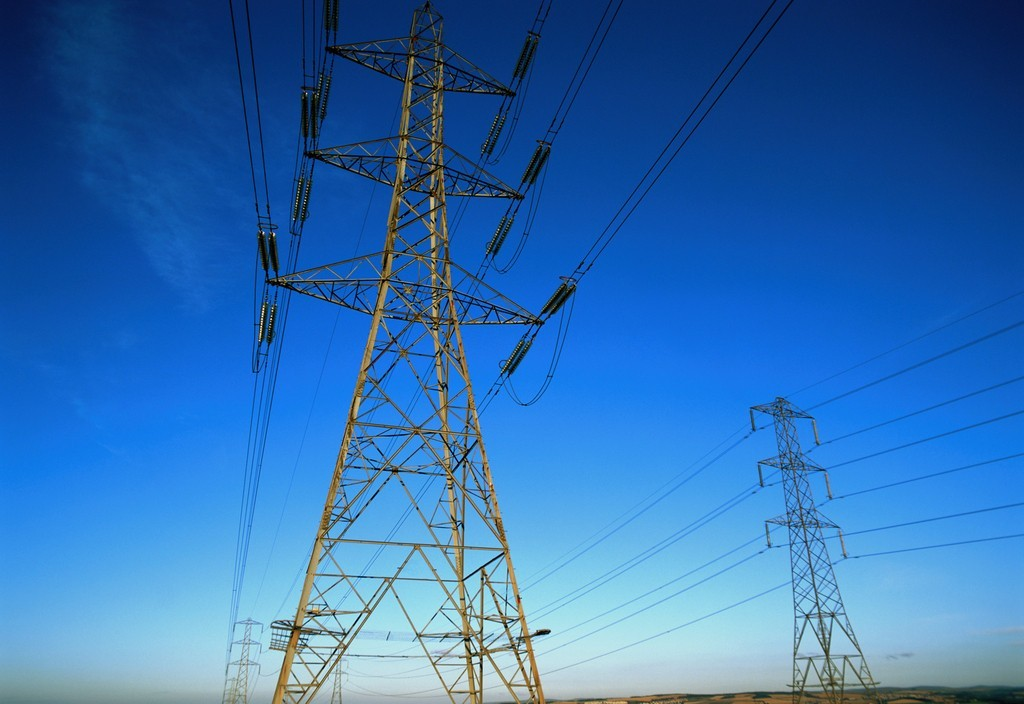
\includegraphics[height=6.5cm]{line.jpg} \
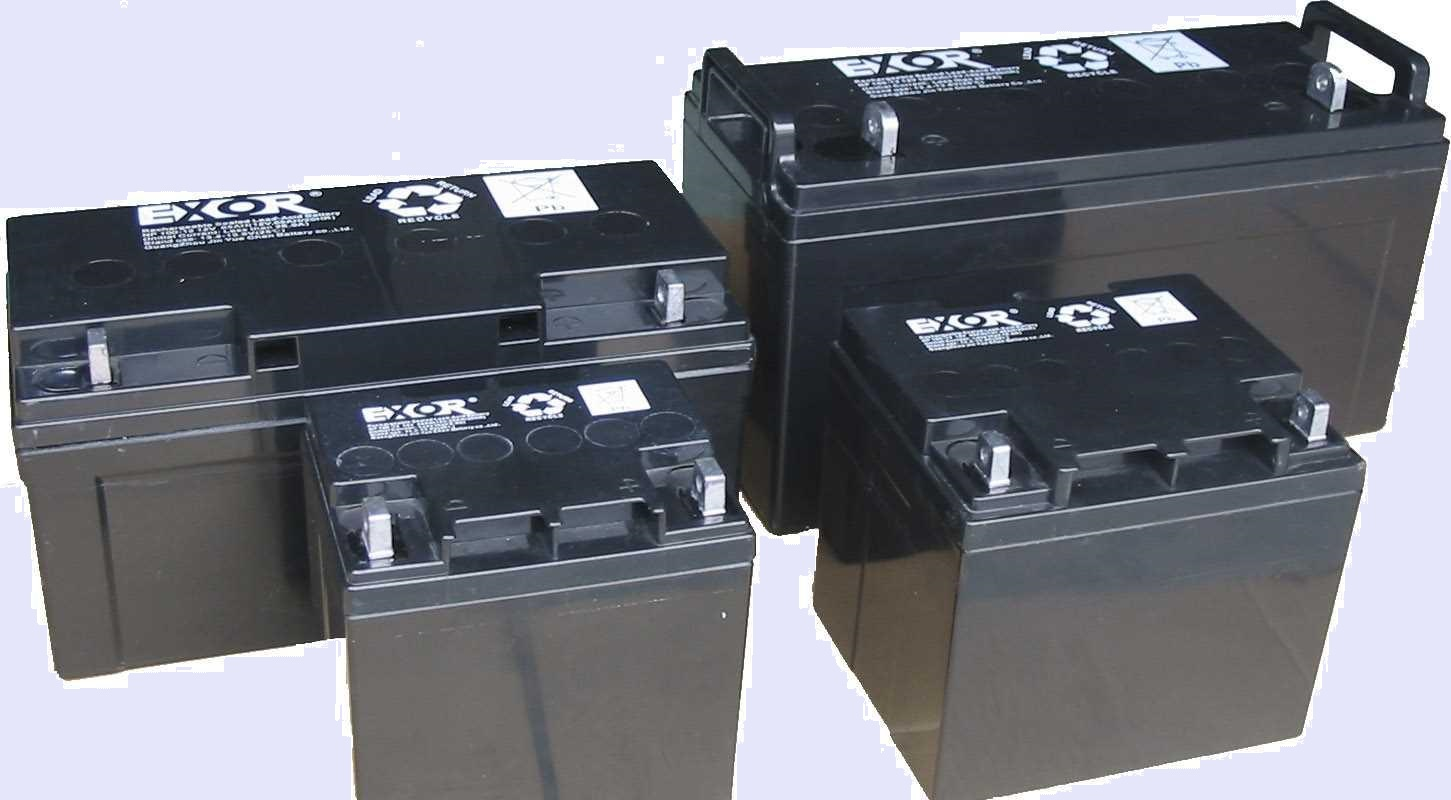
\includegraphics[height=6.5cm]{battery.jpg}\
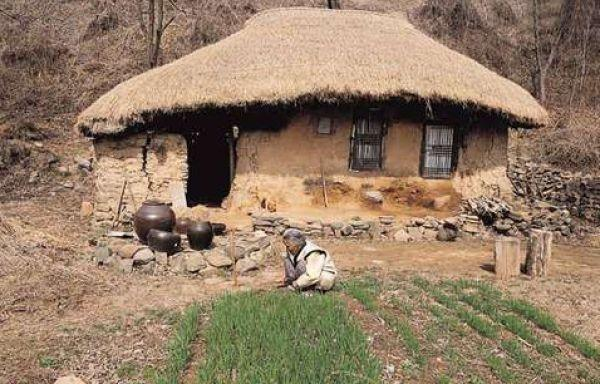
\includegraphics[height=6.5cm]{undev.jpg}\\

\section*{Specification of the problem}

In an undeveloped country where the electricity is only available for about one hour in a day, the organization decides to set up a storage system to provide full-day power to users.

As the grid is on only for a short time in a 
day, the organization fully charges the battery during this time, and discharges it to provide power to users for the rest of the day. 

The  total energy provided to users within the day cannot exceed the capacity, and if the capacity is depleted, a cost 
proportional to the shortage will be imposed on the society. 

This research discusses about strategies for
 deciding on the capacity to minimize the total social cost and charging users in a fair way to cover the construction and running cost of the organization.

\section*{Challenges}

\begin{itemize}

\item \blue{Optimal capacity?} \\
Trade off between efficiency and stability\\ 
  Solution: Investigate users' demand distribution
\item \blue{Limited information} \\
Users do not even know their demands! \\
Solution: Do power-on experiments for data
\item \blue{Optimal sample size?} \\
Larger sample, more sampling cost but less error \\
Solution: High-level estimation based on statistics
\item \blue{How to charge users?} \\
Solution: Compromise between efficiency and fairness

\end{itemize}

\section*{Setting up}



\begin{itemize}



\item Experimentally power $m\ll n$ users among $n$ for demand data
\item Decide on optimal capacity and fully build the system
\item Charge users in a proper standard

\end{itemize}

\section*{Model of Costs}
\begin{itemize}
\item System capacity: $C$
\item Amortized daily cost of storage: $s\cdot C$, proportional to $C$
\item User $i$'s daily demand: $X_i\sim N(\mu_i,\sigma_i^2)$, independent
\item $\sum X_i<C$: sparing cost rate $s$
\item $\sum X_i>C$: shortage penalty rate $\gamma>s$
\item $\sum X_i\sim N(\sum\mu_i, \sum\sigma_i^2)$
\item \blue{Optimal capacity:} \\
\blue{ $$C_* = \sum\mu_i + K_1\sqrt{\sum\sigma_i^2}$$ }
\item Risk-reserving ratio $K_1$ s.t. (from SPP) \\
$$     Q(K_1)=\frac{s}{s+\gamma} $$
in which $Q(\cdot)$ is the gaussian tail probability function
\item Basic capacity:
 $$ C_b = \sum\mu_i $$
\item Risk-reserving capacity:
 $$ C_r = K_1\sqrt{\sum\sigma_i^2} $$
\end{itemize}

\section* {Sample Setting}
\begin{itemize}
\item Sampling cost:
 $$c_{smp}=\Theta(m)$$
\item Sampling deviation of $nE[\mu_i]$ and $nE[\sigma_i^2]$:
 $$\delta_1^{(1)}=\Theta\left(\frac{n}{\sqrt{m}}\right)$$
\item Error between expected sums and actual sums:
 $$\delta_1^{(2)}=\Theta(\sqrt{n})$$
\item Sampling error of parameters:
 \begin{align*}
	\delta_1 &= \delta_1^{(1)} + \delta_1^{(2)} \\
            &= \Theta\left(\frac{n}{\sqrt{m}}\right)
 \end{align*}

\item Demand fluctuation:
 $$\delta_2=\Theta(\sqrt{n})$$
\item For $n\to\infty,m=o(n)$, $\delta_1\gg\delta_2$
\item Error cost: $c_{err}$
\item When $\delta_1\gg\delta_2$:
 $$ c_{err}\sim\delta_1 $$
 $$ $$
\begin{center}
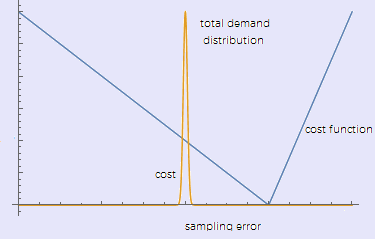
\includegraphics[width=20cm]{error.png}
\end{center}
 $$ $$

The optimal sample size:
\blue{ $$ m_{opt}=\Theta(n^{2/3})$$ }
\item When $\delta_1\ll\delta_2$ (large $E[\sigma_i^2]$, small $n$)

$$ c_{err}\sim\delta_1^2 $$
 $$ m_{opt}\sim n$$

 
\end{itemize}

\section* {Payment Policy}
\begin{itemize}
\item Assume that the organization do not want to make profit, only charge users to cover the cost.
\item Only calculating the additional cost of the system, electricity cost is charged as usual.
\item \blue{Negative externality} of user $i$: $w_i$ s.t.
\begin{align*}
 \frac{\partial w_i}{\partial \mu_i} &= s  \\
 \frac{\partial w_i}{\partial \sigma_i} &= K_1 s \frac{\sigma_i}{\sqrt{nE[\sigma_i^2]}} 
\end{align*}
$$ \implies \blue{w_i=\left(\mu_i+K_1\frac{\sigma_i^2}{2\sqrt{nE[\sigma_i^2]}}\right)s} $$
\item Problem:
\begin{align*}
 \sum w_i &= s\cdot\left( C_b+\frac{1}{2}C_r \right) \\
          &< s\cdot C_*
\end{align*}
---Due to \blue{scale effect: more users, lower marginal cost}

---\red{Cannot cover the cost!}

\item \blue{Alternative 1:}
\blue{$$ w_i^{(1)}=\left(\mu_i+K_1\frac{\sigma_i^2}{\sqrt{nE[\sigma_i^2]}}\right)s $$} \\
---Respecting the cost structure of the system \\
---Realizing \red{fairness of outcome} \\

\item \blue{Alternative 2:} 
\blue{$$ w_i^{(2)}=\left(\mu_i+K_1\frac{\sigma_i \sqrt{nE[\sigma_i^2]}}{nE[\sigma_i]}\right)s $$} \\
---Equivalence under the \blue{Veil of Ignorance} \\
---Realizing \red{fairness of opportunity}

\item \blue{Conflicts between ``fairness''} \\
If I exactly double up my power consumption, should I pay more than double? \\
---Yes, because I am bringing \blue{more than double cost} to the organization. \\
---No, the extra cost \blue{is not my fault}, it comes from some \blue{disadvantage of the system}!

\item {When $n\to\infty$}, as the portion of $C_r$ diminishes with $\frac{1}{\sqrt{n}}$, user $i$'s payment in all policies converges to $\mu_i\cdot s$ \\
\red{When we share more, there will be not only more efficiency, but also fewer conflicts!}


\end{itemize}



\end{multicols}
\end{document}